

\begin{frame}{Chiffrement re-randomizable}

  Exemple: Chiffrement ElGamal
  
  \begin{figure}
    \tiny
    \begin{centering}
      \begin{tikzpicture}
        \node (E) at (0,0)[minimum width = 1.5 cm, minimum height = 1.5cm]{\includegraphics[width = 0.1\textwidth]{images/Alice.png}};
        \node (D) at (6,0)[minimum width = 1.5 cm, minimum height = 1.5cm]{\includegraphics[width = 0.1\textwidth]{images/Bob.png}};
        
        \node (ke) at (0,1.5){Clef de chiffrement $\PK = g^a$};
        \path (ke) edge [->] (E.north);
        \node (kd) at (6,1.5){Clef de d\'echiffrement $\SK = a$};
        \path (kd) edge [->] (D.north);
        
        \node (m) at (-2.5,0.5){Message $m$};
        \path (m) edge [->] ([yshift = 0.5cm]E.west);
        \node (r) at (-2.5,-0.5){Al\'ea $r$};
        \path (r) edge [->] ([yshift = -0.5cm]E.west);

        \pause
        \node (M) at (3,0)[minimum width = 1.5 cm, minimum height = 1.5cm]{\includegraphics[width = 0.1\textwidth]{images/Merlin.jpg}};
        \path (E) edge[->] node[above]{$c$} node[below]{$=\{g^r, m\cdot g^{ar}\}$}(M);
        \path (M) edge [->] node[above]{$c'$} node[below]{$=\{g^{r'}, m \cdot g^{ar'}\}$}(D);
        \node (m3) at (6,-1.5){Message d\'echiffr\'e $m$};
        \path (D) edge [->] (m3);
        
        
      \end{tikzpicture}
    \end{centering}
  \end{figure}

  \pause
  
  \visible<3->{{\color{blue} \emph{Correction}: } $Dec(\SK, Enc(\PK, m, r)) = m$}
  

\end{frame}



%\begin{frame}{Mixnetwork}
%  
%  \begin{figure}
%    \tiny
%    \begin{tikzpicture}
%      \node (People1) at (0,0)[minimum width = 1.5 cm, minimum height = 1.5cm]{\includegraphics[width = 0.1\textwidth]{images/people.png}};
%      \node (Server1) at (2,0)[minimum width = 1.5 cm, minimum height = 1.5cm]{\includegraphics[width = 0.1\textwidth]{images/server.png}};
%      \node (Void) at (4,0)[minimum width = 1.5 cm, minimum height = 1.5cm]{\dots};
%      \node (Server2) at (6,0)[minimum width = 1.5 cm, minimum height = 1.5cm]{\includegraphics[width = 0.1\textwidth]{images/server.png}};
%      \node (People2) at (8,0)[minimum width = 1.5 cm, minimum height = 1.5cm]{\includegraphics[width = 0.1\textwidth]{images/people.png}};
%      \node (SK) at (6,2) {Decryption key $sk$};
%      \path (SK) edge[->] (Server2);
% 
%      \path ([yshift = 0.5cm] People1.east) edge[->] node[above]{$c_1$} ([yshift = 0.5cm] Server1.west);
%      \path ([yshift = 0cm] People1.east) edge[->] node[above]{$c_2$}([yshift = 0cm] Server1.west);
%      \path ([yshift = -0.5cm] People1.east) edge[->] node[above]{$c_3$}([yshift = -0.5cm] Server1.west);
% 
%      \path ([yshift = 0.5cm] Server1.east) edge[->] ([yshift = 0cm] Void.west);
%      \path ([yshift = 0cm] Server1.east) edge[->] ([yshift = -0.5cm] Void.west);
%      \path ([yshift = -0.5cm] Server1.east) edge[->] ([yshift = 0.5cm] Void.west);
%      
%      \path ([yshift = 0.5cm] Void.east) edge[->] ([yshift = -0.5cm] Server2.west);
%      \path ([yshift = 0cm] Void.east) edge[->] ([yshift = 0.5cm] Server2.west);
%      \path ([yshift = -0.5cm] Void.east) edge[->] ([yshift = 0cm] Server2.west);
%      
%      \path ([yshift = 0.5cm] Server2.east) edge[->] node[above]{$m_1$}([yshift = 0.5cm] People2.west);
%      \path ([yshift = 0cm] Server2.east) edge[->] node[above]{$m_2$}([yshift = 0cm] People2.west);
%      \path ([yshift = -0.5cm] Server2.east) edge[->] node[above]{$m_3$}([yshift = -0.5cm] People2.west);
%    \end{tikzpicture}
%  \end{figure}
%\end{frame}

\begin{frame}{Syst\`eme de vote sans re\c{c}u}

  Exemple: ElGamal

  \begin{figure}
    \tiny
    \begin{tikzpicture}
      \node (A) at (0,0)[minimum width = 1.5 cm]{\includegraphics[width=0.1\textwidth]{images/Alice.png}};
      \node (Adv) at (0,3)[minimum width = 1.5 cm]{\includegraphics[width=0.1\textwidth]{images/Eve.png}};
      \node (Gov) at (6,0)[minimum width = 1.5 cm]{\includegraphics[width=0.1\textwidth]{images/government.png}};
      \path (A) edge[->] node[above]{Vote : $c = \{g^r, m\cdot g^{ar}\}$} (Gov);
      \path ([xshift = -0.25cm]Adv.south) edge[->] node[below,sloped]{\tiny Donne-moi une preuve!}([xshift = -0.25cm]A.north);
      \path ([xshift = 0.25cm]A.north) edge[->] node[below,sloped]{\tiny La preuve est $r$.}([xshift = 0.25cm]Adv.south);
      \path (Gov) edge[->] node[above]{Corrompu}(Adv);
    \end{tikzpicture}
   \end{figure}
\end{frame}




\begin{frame}{Syst\`eme de vote sans re\c{c}u}
  \begin{figure}
    \tiny
    \begin{tikzpicture}
      \node (A) at (0,0)[minimum width = 1.5 cm]{\includegraphics[width=0.1\textwidth]{images/Alice.png}};
      \node (Adv) at (0,3)[minimum width = 1.5 cm]{\includegraphics[width=0.1\textwidth]{images/Eve.png}};
      \node (Server) at (3,0)[minimum width = 1.5 cm]{\includegraphics[width=0.1\textwidth]{images/server.png}};
      \node (Gov) at (6,0)[minimum width = 1.5 cm]{\includegraphics[width=0.1\textwidth]{images/government.png}};
      \path (A) edge[->] node[above]{Vote $\{g^r, g^{ar}\}$} (Server);
      \path ([xshift = -0.25cm]Adv.south) edge[->] node[below,sloped]{\tiny Donne-moi une preuve!}([xshift = -0.25cm]A.north);
      \path ([xshift = 0.25cm]A.north) edge[->] node[below,sloped]{\tiny Je ne peux pas!}([xshift = 0.25cm]Adv.south);
      \path (Server) edge[->]node[above]{Votes re-randomiz\'es} node[below]{$\{g^{r'}, g^{ar'}\}$} (Gov);
      \path (Gov) edge[->] node[above]{Corrompu}(Adv);
    \end{tikzpicture}
   \end{figure}
\end{frame}


\begin{frame}{Indistinguishable Chosen-Ciphertext Attack (IND-CCA) et Replayable Chosen-Ciphertext Attack (RCCA)}
  \alt<2->{RCCA}{IND-CCA}
  %  \begin{figure}
  %    \tiny
  %    \begin{centering}
  % 
  %      \begin{tikzpicture}
  % 
  %        \node (A) at (3,0)[draw, thick, minimum width = 1.5 cm, minimum height = 3cm]{\includegraphics[width=0.1\textwidth]{images/Eve.png}};
  %        \node (D) at (6,0)[draw, thick, minimum width = 1.5 cm, minimum height = 3cm]{\includegraphics[width = 0.05\textwidth]{images/Bob.png}};
  %        \node (E) at (0,0)[draw, thick, minimum width = 1 cm, minimum height = 1cm]{\includegraphics[width = 0.05\textwidth]{images/Alice.png}};
  %        
  %        
  %        \node (mb) at (-2,0.25){$b$};
  %        \path (mb) edge [->] ([yshift = 0.25cm]E.west);
  %        \node (r) at (-2,-0.25){$r$};
  %        \path (r) edge [->] ([yshift = -0.25cm]E.west);
  % 
  %        \path (E) edge[->] node[above]{$c^* = Enc(m_b; r)$}(A);
  % 
  %        \path ([yshift = 1.25cm]A.east) edge[->] node[above]{$\{c_i\}$}([yshift = 1.25cm]D.west);
  %        \path ([yshift = 0.75cm]A.east) edge[<-] node[above]{$\{m_i\}$}([yshift = 0.75cm]D.west);
  %        
  %        \path ([yshift = -0.75cm]A.east) edge[->] node[above]{\alt<2>{Cond\footnote{$Dec(k_d, \{c_j\}) \not \in \{m_0,m_1\}$}}{$\{c_j\}\neq c^*$}}([yshift = -0.75cm]D.west);
  %        \path ([yshift = -1.25cm]A.east) edge[<-] node[above]{$\{m_j\}$}([yshift = -1.25cm]D.west);
  %        
  %        
  %        \node (b') at (1,-1){$b'$};
  %        \path ([yshift= -1cm]A.west) edge[->] (b');
  % 
  %        
  %        \node (ke) at (3,2.5){$k_e$};
  %        \path (ke) edge[->](A);
  %        \node (kd) at (6,2.5){$k_d$};
  %        \path (kd) edge[->](D);
  %        
  %        \node (m0) at (1.5,1.25){$m_0$};
  %        \path ([yshift = 1.25cm]A.west) edge[->] (m0);
  %        \node (m1) at (1.5,0.75){$m_1$};
  %        \path ([yshift = 0.75cm]A.west) edge[->] (m1);
  % 
  % 
  %        \node (def)[align=left] at (-3,2){$b\in\{0,1\}$, $r$ random \\ $|r| = |m_0| = |m_1|$ \\ $i \in Query1$ \\ $j \in Query2$};
  %      \end{tikzpicture}
  % 
  %    \end{centering}
  %  \end{figure}

  \begin{figure}
    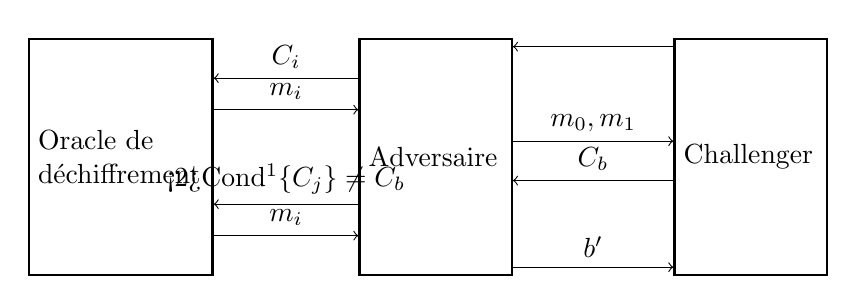
\begin{tikzpicture}
      \node(A)[draw, thick, text width = 1.7cm, minimum height = 3cm] at (0,0) {Adversaire};
      \node(C)[draw, thick, text width = 1.7cm, minimum height = 3cm] at (4,0) {Challenger};
      \node(D)[draw, thick, text width = 2.1cm, minimum height = 3cm] at (-4,0) {Oracle de d\'echiffrement};
      
      \path([yshift = 1.4cm]A.east) edge[<-] node[above]{$\PK$} ([yshift = 1.4cm]C.west);
      \path([yshift = 1cm]D.east) edge[<-] node[above]{$C_i$} ([yshift = 1cm]A.west);
      \path([yshift = 0.6cm]D.east) edge[->] node[above]{$m_i$} ([yshift = 0.6cm]A.west);
      \path([yshift = 0.2cm]A.east) edge[->] node[above]{$m_0, m_1$} ([yshift = 0.2cm]C.west);
      
      \path([yshift = -0.3cm]A.east) edge[<-] node[above]{$C_b$}([yshift = -0.3cm]C.west);
      \path([yshift = -0.6cm]D.east) edge[<-] node[above]{\alt<2>{Cond\footnote{$Dec(k_d, \{C_j\}) \not \in \{m_0,m_1\}$}}{$\{C_j\}\neq C_b$}} ([yshift = -0.6cm]A.west);
      \path([yshift = -1cm]D.east) edge[->] node[above]{$m_i$} ([yshift = -1cm]A.west);
      
      \path([yshift = -1.4cm]A.east) edge[->] node[above]{$b'$}([yshift = -1.4cm]C.west);
    \end{tikzpicture}
    
  \end{figure}

  {\color{blue} Advantage:} $Adv(\Adv) = |\PR[b = b'] - \frac{1}{2}|$.
\end{frame}
